\documentclass[times,final]{elsarticle}
%%
%\documentclass[times,twocolumn,final,longtitle]{elsarticle}
%%
%% Compress citation scheme
\biboptions{numbers,sort&compress}

%% Stylefile to load JCOMP template
\usepackage{jcomp}
\usepackage{framed,multirow}

%% The amssymb package provides various useful mathematical symbols
\usepackage{mathrsfs}
\usepackage[fleqn]{amsmath}
\usepackage{amssymb}
\usepackage{latexsym}

% Following three lines are needed for this document.
% If you are not loading colors or url, then these are
% not required.
\usepackage{url}
\usepackage{xcolor}
\definecolor{newcolor}{rgb}{.8,.349,.1}

%% Define a new 'leo' style for the package that will use a smaller font.
\makeatletter
\def\url@leostyle{%
  \@ifundefined{selectfont}{\def\UrlFont{\sf}}{\def\UrlFont{\small\ttfamily}}}
\makeatother

%% Now actually use the newly defined style.
\urlstyle{leo}

%%insert figures
\usepackage{caption}
\usepackage{graphicx}
\usepackage{epstopdf}
%\usepackage{graphicx,times}
\usepackage{subfigure}
\usepackage{natbib}
\usepackage{geometry}
%\geometry{left=2cm,right=2cm,top=2cm,bottom=2cm}
\graphicspath{{pictures/}}
\journal{Journal of Computational Physics}
\begin{document}
\verso{Given-name Surname \textit{etal}}

\begin{frontmatter}

\title{A coupled level set and volume of fluid method for sharp interface simulation}%

\author[1]{Linfan \snm{Zhang}\corref{cor1}}
\cortext[cor1]{Corresponding author:
  Tel.: +0-000-000-0000;
  fax: +0-000-000-0000;}
\author[1]{Weimin \snm{Ma}\fnref{fn1}}
%\fntext[fn1]{This is author footnote for second author.}
%\author[2]{Arthur \snm{Morgan}}
%% Third author's email
\ead{zlf0030@163.com}
%\author[2]{Edward \snm{Conway}}

\address[1]{Affiliation 1, Address, City and Postal Code, China}
\address[2]{Affiliation 2, Address, City and Postal Code, Country}

\received{1 Jan 2019}
\finalform{10 Jan 2019}
\accepted{13 Jan 2019}
\availableonline{15 Jan 2019}
%\communicated{S. Sarkar}


\begin{abstract}
 This paper presents a coupled level-set and volume-of-fluid method for unstructured meshes. This method designed for simulating incompressible two phase flows combines both the advantages of LS method and VOF method. The method is called CLSAdvector, and is implemented into OpenFOAM$^{\textregistered}$ as open source. Volume of fluid (VOF) idea is conservative because it can calculate the volume of one of the fluids transported across the mesh faces in a time step. In contrast to VOF, the LS method provides a sharp interface and a smooth transition in the physical properties across the interface. The novelty of the CLSAdvector concept combines the ideas of VOF and LS method. First, an algorithm is designed for calculating the position of interface inside cells where the void fraction and the direction of interface are given. Second, the level set function is limited in a narrow band that contains the interface, which improves the efficiency of the algorithm. The feasibility and accuracy of the current method are validated by several cases including Zalesak's problem, 2D vortex, dam break, and jet break-up.
\end{abstract}
\begin{keyword}
interfacial flows\sep CLSAdvection \sep CFD \sep OpenFOAM$^{\textregistered}$
%\KWD Keyword1\sep Keyword2\sep Keyword3
\end{keyword}

\end{frontmatter}

\input{section1}
\input{section2}
\section{Numerical implementations}
\subsection{Cutting the cell with $\alpha$ and $\phi$}
In this case, the normal direction $\mathbf{n}$ of certain cell is given by level set function $\phi$ and the void fraction $\alpha$ is given by volume of fluid function. This section means to explain the algorithm of finding such a plane with normal direction $\mathbf{n}$ that can cut the cell into the right void fraction $\alpha$. The locations of cell center point $\mathbf{x_i}$ and $N$ cell vertexes $\mathbf{x_{i_1}},...,\mathbf{x_{i_N}}$ are needed. Then we can get $N$ vectors $\mathbf{d_1},...,\mathbf{d_N}$ from cell center to $N$ cell vertexes. The projections of center point to vertex on the normal direction can be calculated as
\begin{equation}\label{21}
D_i=\mathbf{d_i}\cdot\mathbf{n},\quad for\quad i=1,...,N.
\end{equation}
Let us suppose the objective plane contain one of the vertexes and we can have a series of plane to cut the cell into different fractions (figure \ref{fig:multiplane}). Due to the cell's polyhedral characteristic, a piecewise function about the center cell distance and void fraction is drew in figure \ref{fig:piecewise}. The objective plane with the given void fraction $\alpha_i$ must have a certain distance $D^*$ to the center point $\mathbf{x_i}$ such that $\tilde{\alpha}(D^*)=\alpha_i $ .The first step is to find the point on the certain part of the piecewise function, which can be realized by comparing the void fraction value of vertexes and $\alpha^*$. Suppose the point $p$ is between point $k$ and $l$, such that ${D^*}\in[D_k,D_l]$. We use a cubic polynomial to fit this interval. The second step is to find the two trisection point in this interval, say, $m$ and $n$, and calculate the $\tilde{\alpha}(D_m)$ and $\tilde{\alpha}(D_n)$ in geometric way. Then we have four points for the four polynomial coefficients by solving a group of linear equations. Use LU decomposition to solve the linear $4\times4$ Vandermonde matrix system. Then use Newton's root finding method to find $D^*$ with the condition, $\left|\tilde{\alpha}(D^*)-\alpha_i\right|<\epsilon$. $\epsilon$ is a user-defined tolerance, typically set to $10^{-8}$.

\begin{figure}[htbp]
\centering
\subfigure[]{
\centering
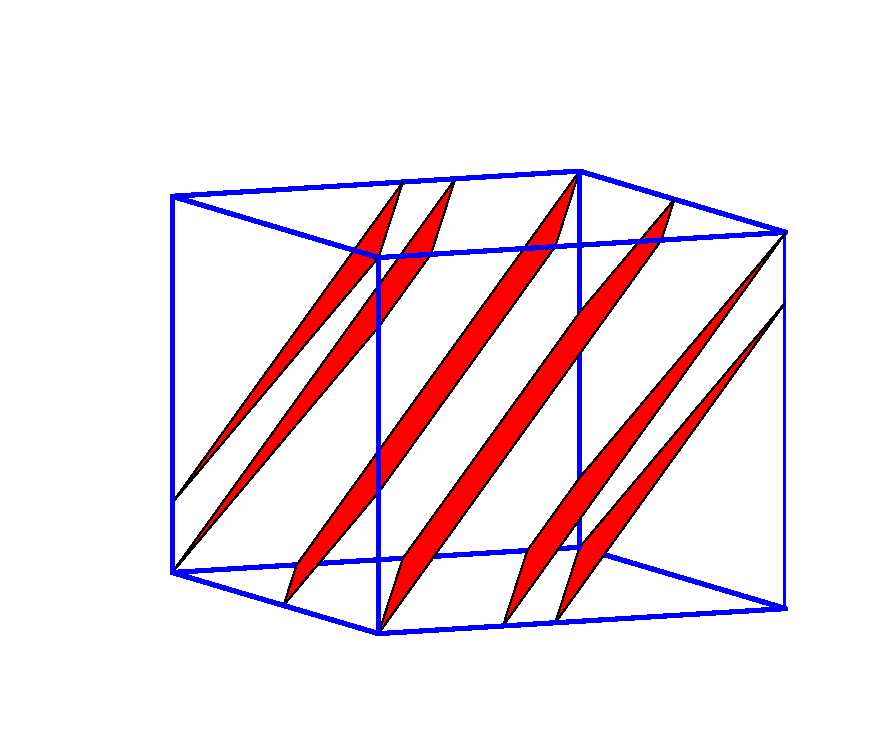
\includegraphics[width=0.4\textwidth]{multiplane.eps}
%\caption{fig1}
\label{fig:multiplane}
}
\quad
\subfigure[]{
\centering
\includegraphics[width=0.4\textwidth]{piecewisefunction.eps}
\label{fig:piecewise}
%\caption{fig2}
}
%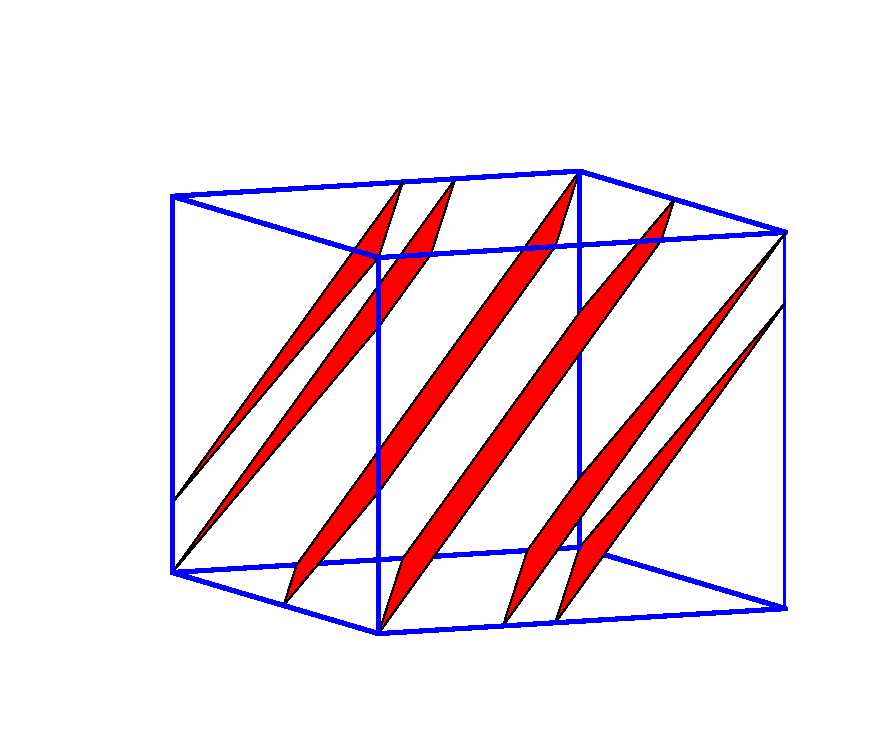
\includegraphics [width=0.5\textwidth]{multiplane.eps}
\caption{\subref{fig:multiplane} shows that planes pass different vertexes with the same normal direction. \subref{fig:piecewise} shows the cut volume and distance to the plane.}
\label{fig:multi}
\end{figure}

\subsection{Narrow band containing interface}
The cells that contain the interface are limited to where $\alpha\in(\xi,1-\xi)$. $\xi$ is defined by users to confine the algorithm resolution, usually set as $0.01$. However, only interface cells are not enough to reconstruct the details of the interface. Level set method needs to build the signed distance function in the whole field, which can precisely capture the interface but take too much computational resource and time. So it is necessary to build a narrow band that has a thickness of two layers of grid like figure(\ref{•}). The first step is to sign all the interface cells with the flag "seed". The second step is to 

\subsection{Reinitialization}

\subsection{Correction for mass conservation}

\subsection{Numerical Discretization of level set equation}


\section{Results}
In the following, some test cases with CLSAdvection method are presented. It is known that level set method can improve the sharpness of the interface but cause mass loss while the volume of fluid method just keep the interface mass conservative but smeared. Therefore, the validation of the CLSAdvection method is tested and there are several simple cases comparing this coupled method with the level set method and volume of fluid method. The error measures will be used to quantify the solution quality with following aspects.
1. Mass conservation
\begin{equation}\label{29}
\varepsilon_{M}(t)=\frac{\left|\sum\limits^N_{i=1}\rho_i(t)V_i-\sum\limits_{i=1}^N\rho_i(0)V_i\right|}{\sum\limits^N_{i=1}\rho_i(0)V_i}.
\end{equation}
2. Volume conservation
The fractional volume conservative error is defined as following equation by this article\cite{gopala2008volume},
\begin{equation}\label{28}
\varepsilon_{V}(t)=\frac{\left|\sum\limits^N_{i=1}\alpha_i(t)V_i-\sum\limits^N_{i=1}\alpha_i(0)V_i\right|}{\sum\limits^N_{i=1}\left|\alpha_{i}(0)V_i\right|}
\end{equation}
3.
\subsection{Zalesak's test problem}
Solid body rotation of a notched disc is commonly used to test the advection capabilities of an interface capture solver. Zalesak firstly introduced this test \citep{zalesak1979fully} and its variants have been used extensively. In this particular test, the radius of the disc is $R=0.15$, the notch width is $W=0.06$ and the notch height is $H=0.25$. The center of the disc lies in $(x_0,y_0)=(0.5,0.75)$ in a domain of $1\times{1}$ that is discretized using a rectangular mesh of size $100\times{100}$. The rotation velocity is given by 
\begin{equation}\label{27}
\begin{split}
&u=-2\pi(y-0.5)
\\
&v=2\pi(x-0.5).
\end{split}
\end{equation}
At all the domain boundary, zero gradient condition is set for $\alpha$ and $\phi$. 



\subsection{Spiralling disc}

\subsection{Dambreak}

%\subsection{Droplet distortion}

%\subsection{Jet break up}
\input{section5}

%%Vancouver style references.
\bibliographystyle{model1-num-names}
\bibliography{refs}

%\section*{Supplementary Material}

\end{document}

%%
